% Figure 1: flow of records (shell). Every count is left as a dash until the records have been screened and coded.
\documentclass[border=4pt]{standalone}
\usepackage[T1]{fontenc}
\usepackage{lmodern}
\usepackage{tikz}
\usetikzlibrary{positioning,arrows.meta}
\begin{document}
\sffamily\small\hyphenpenalty=10000
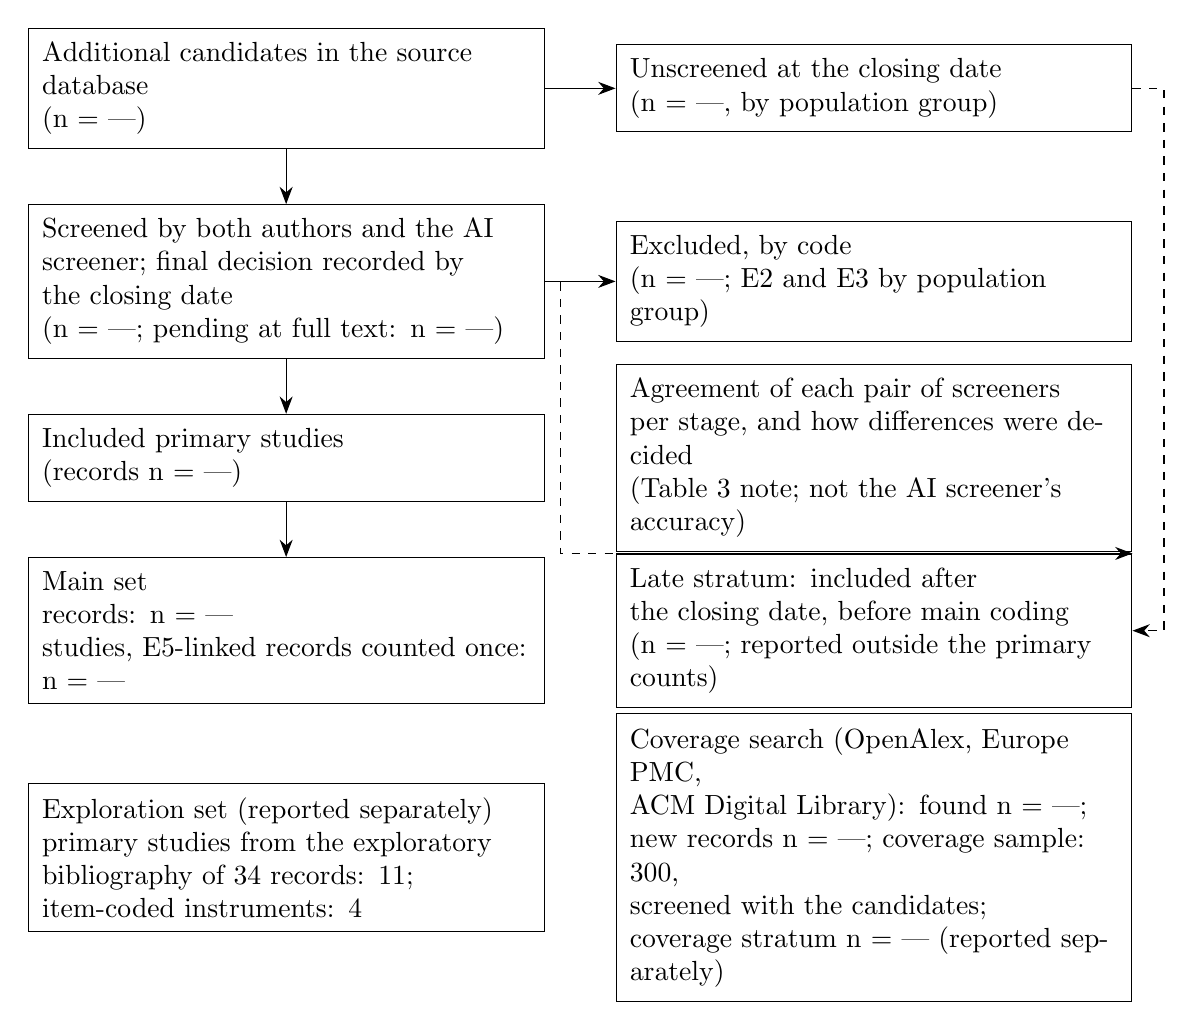
\begin{tikzpicture}[
  box/.style={draw, align=left, text width=62mm, inner sep=5pt},
  side/.style={draw, align=left, text width=62mm, inner sep=5pt},
  arr/.style={-{Stealth[length=2.2mm]}},
  node distance=7mm and 9mm]
  \node[box] (cand) {Additional candidates in the source database\\(n = ---)};
  \node[side, right=of cand] (unscr) {Unscreened at the closing date\\(n = ---, by population group)};
  \node[box, below=of cand] (scr) {Screened by both authors and the AI\\screener; final decision recorded by\\the closing date\\(n = ---; pending at full text: n = ---)};
  \node[side, right=of scr] (excl) {Excluded, by code\\(n = ---; E2 and E3 by population group)};
  \node[box, below=of scr] (incl) {Included primary studies\\(records n = ---)};
  \node[side, right=of incl] (agree) {Agreement of each pair of screeners\\per stage, and how differences were decided\\(Table~3 note; not the AI screener's\\accuracy)};
  \node[box, below=of incl] (main) {Main set\\records: n = ---\\studies, E5-linked records counted once:\\n = ---};
  \node[side, right=of main] (late) {Late stratum: included after\\the closing date, before main coding\\(n = ---; reported outside the primary counts)};
  \node[box, below=10mm of main] (expl) {Exploration set (reported separately)\\primary studies from the exploratory\\bibliography of 34 records: 11;\\item-coded instruments: 4};
  \node[side, right=of expl] (cov) {Coverage search (OpenAlex, Europe PMC,\\ACM Digital Library): found n = ---;\\new records n = ---; coverage sample: 300,\\screened with the candidates;\\coverage stratum n = --- (reported separately)};
  \draw[arr] (cand) -- (scr);
  \draw[arr] (cand) -- (unscr);
  \draw[arr] (scr) -- (incl);
  \draw[arr] (scr) -- (excl);
  \draw[arr] (incl) -- (main);
  \draw[arr, dashed] (unscr.east) -- ++(4mm,0) |- (late.east);
  \draw[arr, dashed] (scr.east) -- ++(2mm,0) |- (late.north east);
\end{tikzpicture}
\end{document}
